{}

\section{{Problem 1}}

	\subsection{{Computer Program}}

		\begin{lstlisting}[language=C, caption=\textit{Hello World Program}]	
/*  Program to calculate the Training Heart Rate (THR)  */

#include <stdio.h>
#include <math.h>
#include <stdbool.h>

float inputs(void);
bool gender_conditional(char gender);
int male_training_heart_rate(int age, int resting_heart_rate, float fitness_level);
int female_training_heart_rate(int age, int resting_heart_rate, float fitness_level);
int conditional(char gender, int age, int resting_heart_rate, float fitness_level);
void output(int training_heart_rate);

void main(void)
{
    float g, a, rhr, fl = inputs();
    int thr = conditional(g, a, rhr, fl);
    output(thr);
}

float inputs(void)
{
    char gender;
    int age;
    int resting_heart_rate;
    float fitness_level;

    /*  Scanning values for gender selection    */
    printf("Please enter your gender, (M or F): ");
    do
    {
        scanf("%c", &gender);
    } while (gender == 'M' || gender == 'F');
    

    /*  Scanning values for the age */
    printf("\nPlease enter your age: ");
    scanf("%i", &age);

    /*  Scanning values for the resting heart rate  */
    printf("\nPlease enter your resting heart rate: ");
    scanf("%i", &resting_heart_rate);

    /*  Scanning values for fitness level   */
    printf("\nPlease enter your fitness level, (0.55 for low, 0.65 for medium, and 0.8 for high fitness): ");
    scanf("%f", &fitness_level);

    return gender, age, resting_heart_rate, fitness_level;
}

int conditional(char gender, int age, int resting_heart_rate, float fitness_level)
{
    /*  Conditional to check male or female */
    bool binary = gender_conditional(gender);

    /*  Conditional for check male or female THR    */
    int training_heart_rate;
    if (binary == true)
    {
        training_heart_rate = male_training_heart_rate(age, resting_heart_rate, fitness_level);
    }

    else
    {
        training_heart_rate = female_training_heart_rate(age, resting_heart_rate, fitness_level);
    }

    return training_heart_rate;
}

void output(int training_heart_rate)
{
    printf("\nYour training heaty rate is %i\n", training_heart_rate);
}

bool gender_conditional(char gender)
{
    int binary;
    if (gender == 'M')
    {
        binary = true;
    }

    else
    {
        binary = false;
    }
    
    return binary;
}

int male_training_heart_rate(int age, int resting_heart_rate, float fitness_level)
{
    /*  Calculating the maximum heart rate  */
    float maximum_heart_rate = 203.7 / (1 + exp(0.033 * (age - 104.3)));

    /*  Calculating the training heart rate */
    int training_heart_rate = (maximum_heart_rate - resting_heart_rate) * fitness_level + resting_heart_rate;

    return training_heart_rate;
}

int female_training_heart_rate(int age, int resting_heart_rate, float fitness_level)
{
    /*  Calculating the maximum heart rate  */
    int maximum_heart_rate = 190.2 / (1 + exp(0.0453 * (age - 107.5)));

    /*  Calculating the training heart rate */
    int training_heart_rate = (maximum_heart_rate - resting_heart_rate) * fitness_level + resting_heart_rate;

    return training_heart_rate;
}




\end{lstlisting}

	\subsection{{Program Output Screenshot}}

		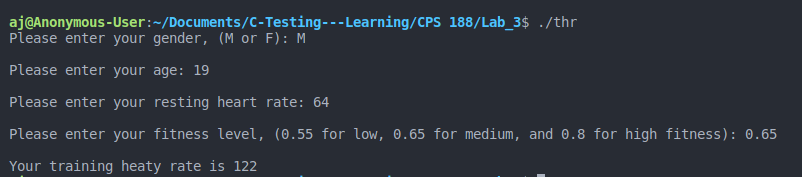
\includegraphics[width=15cm]{thr.png}
		
\section{{Problem 2}}
	
		\subsection{{Computer Program}}
	
			\begin{lstlisting}[language=C, caption=\textit{Program to Calculate the Body Mass Index (BMI) of a person}]	
#include <stdio.h>
#include <math.h>
#include <stdbool.h>

float weight_input(void);
float height_input(void);
void output(float weight, float height);

void main(void)
{
    float w = weight_input();
    float h = height_input();
    output(w, h);
}

float weight_input(void)
{
    float weight;

    /*  Scanning values for weight  */
    printf("Enter your weight: ");
    scanf("%f", &weight);

    return weight;
}

float height_input(void)
{
    float height;

    /*  Scanning values for height  */
    printf("\nEnter your height: ");
    scanf("%f", &height);

    return height;
}

void output(float weight, float height)
{
    /*  Calculating BMI */
    height *= height;
    float body_mass_index = weight / (height);

    /*  Conditional */
    if (body_mass_index < 18.5)
    {
        printf("Your BMI value is %.1f, which classifies you as Underweight\n", body_mass_index);
    }
    else if (body_mass_index <= 24.9)
    {
        printf("Your BMI value is %.1f, which classifies you as Normal\n", body_mass_index);
    }
    else if (body_mass_index <= 29.9)
    {
        printf("Your BMI value is %.1f, which classifies you as Overweight\n", body_mass_index);
    }
    else
    {
        printf("Your BMI value is %.1f, which classifies you as Obese\n", body_mass_index);
    }
}
	\end{lstlisting}

		\subsection{{Program Output Screenshot}}
			
			{}
			
			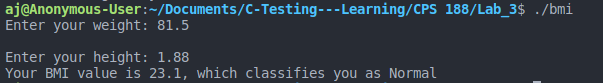
\includegraphics[width=12.75cm]{bmi.png}


\section{{Problem 3}}
	
	\subsection{{Computer Program}}
	
		\begin{lstlisting}[language=C, caption=\textit{Program to Calculate the Overall grades of a Course}]	
/*  Program to Calculate the Overall grades of a Course */

#include <stdio.h>
#include <math.h>

float quiz(void);
float midterm(void);
float final(void);
float conditional_output(float quiz, float midterm, float final);

void main(void)
{
    float q = quiz();
    float m = midterm();
    float f = final();
    conditional_output(q, m, f);
}

float quiz(void)
{
    float quiz[10];
    float lowest;
    float sum = 0;

    printf("Enter your quiz marks (0 to 10):\n");
    for (int i = 0; i < 10; i++)
    {
        do
        {
            scanf("%f", &quiz[i]);
            printf("\n");
        } while (quiz[i] < 0 || quiz[i] > 10);
    }
    
    for (int i = 0; i < 10; i++)
    {
        if (quiz[i] < quiz[i+1])
        {
            lowest = quiz[i];
        }
    }
    
    for (int i = 0; i < 10; i++)
    {
        sum += quiz[i];
    }
    
    float average = (sum - lowest) / 9;

    return average;
}

float midterm(void)
{
    float marks;

    printf("Enter your midterm marks (0 to 100):\n");
    do 
    {
        scanf("%f", &marks);
        printf("\n");
    } while (marks < 0 || marks > 100);

    return marks;
}

float final(void)
{
    float marks;

    printf("Enter your final marks (0 to 100):\n");
    do 
    {
        scanf("%f", &marks);
        printf("\n");
    } while (marks < 0 || marks > 100);

    return marks;
}

float conditional_output(float quiz, float midterm, float final)
{
    quiz *= 0.25;

    if (midterm >= final)
    {
        midterm *= 0.35;
        final *= 0.4;
    }
    else
    {
        midterm *= 0.25;
        final *= 0.5;
    }

    float grade = quiz + midterm + final;

    printf("The overall grade of the course is %.2f\n", grade);
}

	\end{lstlisting}
	
	\subsection{{Program Output Screenshot}}
	
		{}
		
		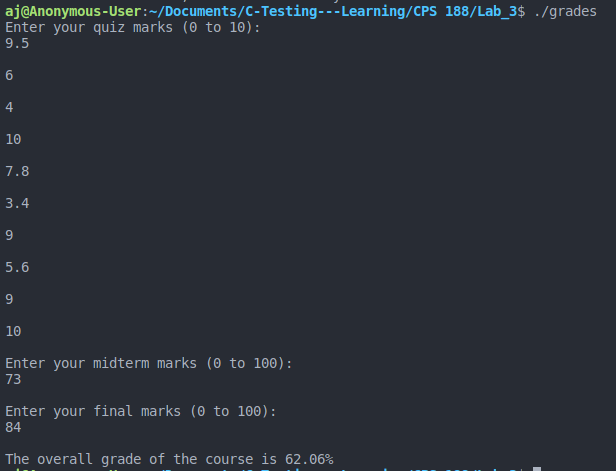
\includegraphics[width=12.75cm]{grades.png}
		
		
		